% Basic stuff
\documentclass[a4paper,10pt]{article}
\usepackage[utf8]{inputenc}
\usepackage[nswissgerman]{babel}
\usepackage{scrextend}
\usepackage{lipsum}
\usepackage{gauss}
\usepackage{amssymb} % to import \leadsto
\usepackage{bookmark}
% 3 column landscape layout with fewer margins
\usepackage[landscape, left=0.75cm, top=1cm, right=0.75cm, bottom=1.5cm, footskip=15pt]{geometry}
\usepackage{flowfram}
\usepackage{floatrow}
\usepackage{amsmath}
\usepackage[inline]{enumitem}
\usepackage{tikz}
\usepackage{tikz-cd} 
\usepackage{multicol}

\usetikzlibrary{calc,matrix}

\changefontsizes[9pt]{8pt}
\ffvadjustfalse
\setlength{\columnsep}{1cm}
\Ncolumn{3}
\DeclareMathOperator{\Tr}{Tr}
\DeclareMathOperator{\Sign}{sign}
\DeclareMathOperator{\Rank}{Rank}
\DeclareMathOperator{\Image}{Im}
\DeclareMathOperator{\Columnspace}{\mathcal{R}}
\DeclareMathOperator{\Nullspace}{\mathcal{N}}
\DeclareMathOperator{\Kernel}{Ker}
\DeclareMathOperator{\diag}{diag}
\DeclareMathOperator{\Span}{span}


% define nice looking boxes
\usepackage[most]{tcolorbox}

% a base set, that is then customised
\tcbset {
  base/.style={
    boxrule=0mm,
    leftrule=1mm,
    left=1.75mm,
    arc=0mm, 
    fonttitle=\bfseries, 
    colbacktitle=black!10!white, 
    coltitle=black, 
    toptitle=0.75mm, 
    bottomtitle=0.25mm,
    title={#1}
  }
}

\newcommand{\middot}{~\textperiodcentered~}
\newlist{rowlist}{enumerate*}{1}
\setlist[rowlist]{label={\textbf{\roman*}\text{: }}, afterlabel={}, itemjoin=\middot}

\newlist{vaxioms}{enumerate*}{1}
\setlist[vaxioms]{label={\textbf{V\arabic*}\text{: }}, afterlabel={}, itemjoin=\middot}

\makeatletter
\renewcommand*\env@matrix[1][*\c@MaxMatrixCols c]{%
  \hskip -\arraycolsep
  \let\@ifnextchar\new@ifnextchar
  \array{#1}}
\makeatother

\newcommand\undermat[2]{%
  \makebox[0pt][l]{$\smash{\underbrace{\phantom{%
    \begin{matrix}#2\end{matrix}}}_{\text{$#1$}}}$}#2}

\newcommand\overmat[2]{%
  \makebox[0pt][l]{$\smash{\overbrace{\phantom{%
    \begin{matrix}#2\end{matrix}}}^{\text{$#1$}}}$}#2}

\definecolor{brandblue}{rgb}{0.34, 0.7, 1}
\newtcolorbox{mainbox}[1]{
  colframe=brandblue, 
  base={#1}
}

\newtcolorbox{subbox}[1]{
  colframe=black!20!white,
  base={#1}
}

% Mathematical typesetting & symbols
\usepackage{amsthm, mathtools, amssymb} 
\usepackage{marvosym, wasysym}
\allowdisplaybreaks

% Tables
\usepackage{tabularx, multirow}
\usepackage{booktabs}

% Make enumerations more compact
\usepackage{enumitem}
\setitemize{itemsep=0.5pt}
\setenumerate{itemsep=0.75pt}

% To include sketches & PDFs
\usepackage{graphicx}

% For hyperlinks
\usepackage{hyperref}
\hypersetup{
  colorlinks=true
}

% Metadata
\title{Cheatsheet Lineare Algebra}
\author{Thomas Gassmann}
\date{August 2022}

% Math helper stuff
\def\limn{\lim_{n\to \infty}}
\def\limxo{\lim_{x\to 0}}
\def\limxi{\lim_{x\to\infty}}
\def\limxn{\lim_{x\to-\infty}}
\def\sumk{\sum_{k=1}^\infty}
\def\sumn{\sum_{n=0}^\infty}
\def\R{\mathbb{R}}
\def\C{\mathbb{C}}
\def\E{\mathbb{E}}
\def\K{\mathbb{K}}
\def\dx{\text{ d}x}

\newcommand{\overbar}[1]{\mkern 1.5mu\overline{\mkern-1.5mu#1\mkern-1.5mu}\mkern 1.5mu}

\begin{document}



\section{The digital image}
A digital image is a discrete representation of a continuous 2D function $I(x,y)$. In sensors the analog digital has to be converted by an ADC (analog to digital converter). 
During exposure the photons are accumulated in the sensor wells, with the accumulated charge being transferred line-by-line to the sense amplifiers which
then pass the signal to the ADC. In CMOS sensors each pixel has its own amplifier and ADC.\\
If we're sampling a signal with a frequency $f_s$ we can only uniquely capture signals with frequencies up to $f_s/2$ (Nyquist frequency). 
To reconstruct a continuous signal from the sample we could use biliner iterpolation:
$$\hat{f}(x, y) = (1 - a)(1 - b)F_{i,j} + a(1 - b)F_{i+1,j} + abF_{i+1,j+1} + (1 - a)bF_{i,j+1}$$
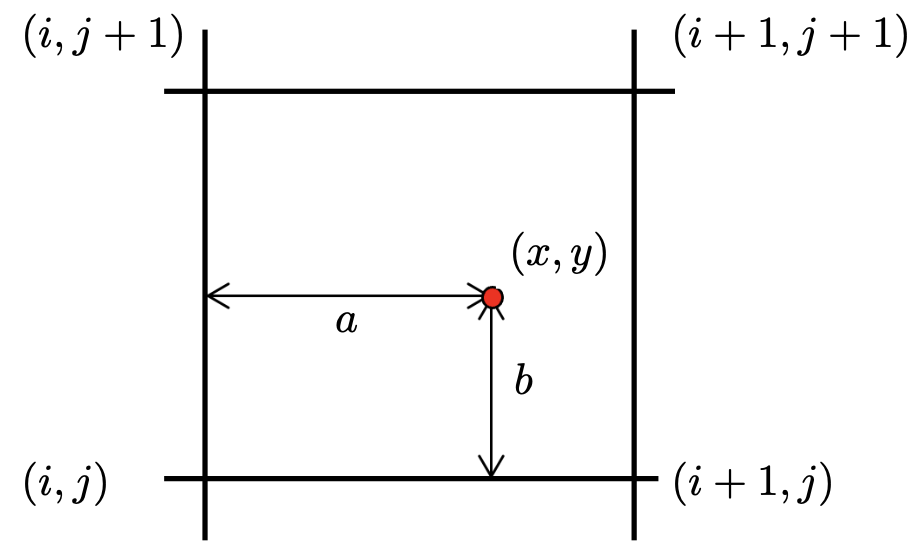
\includegraphics[width=0.6\columnwidth]{bilinear_interplation.png}
\begin{subbox}{Noise ($\sigma$)}
\begin{itemize}
    \item \textbf{Additive Gaussian Noise:} This assumes that the noise follows a normal distribution, i.e. $\tilde{F} - F = \sigma \sim \mathcal{N}(0, \tilde{\sigma}^2)$
    
    \item \textbf{Multiplicative Noise:} Here, the noise follows the intensity of the original signal: $\tilde{F} - F = \sigma = F * c, \quad c \sim \mathcal{N}(b, \tilde{\sigma}^2)$
    
    \item \textbf{Poisson noise (shot noise):} To model scene-dependent noise, the poisson distribution can be used: $p(k) = \frac{\lambda^k e^{-\lambda}}{k!}$, where $\lambda$ is the signal average. Note that for large averages, the poisson distribution is similar to a gaussian distribution.
    
    \item \textbf{Salt-and-Pepper-Noise:} Random black and white pixels are typically caused by faulty sensors or memory errors, hard to describe mathematically, easily removed with median filter.
  
\end{itemize}
There are a number of statistics that aim to quantify noise over an image. Among these, the most popular statistics are:

\begin{itemize}
    \item \textbf{Signal-to-Noise-Ratio (SNR):} $\sigma_{SNR} = \frac{E[F]}{E[\sigma]}$. Because of its wide dynamic range, it is often reported in decibel (dB).
    
    \item \textbf{Peak Signal-to-Noise-Ratio (PSNR):} $\sigma_{SNR} = \frac{F_{max}}{E[\sigma]}$. For most images, $F_{max}$ is 255.
\end{itemize}
\end{subbox}
\section{Image Segmentation}
Classicfication problem where we partition image into disjoint segments.
\subsection{Thresholding}
Choose a threshold $T$ and classify pixels as foreground or background depending on whether their intensity is above or below $T$. For color images, use distance in color space instead of intensity to gage similarity.
\begin{align*}
  B(x,y) &= \begin{cases} 1 & \text{if } I(x,y) > T \\ 0 & \text{else} \end{cases} &&\text{(Grayscale)}\\
  B(x,y) &= \begin{cases} 1 & \text{if } \|(I(x,y), (r,g,b)_{\text{ref}})\|_2 > T \\ 0 & \text{else} \end{cases} &&\text{(Color)}
\end{align*}
Instead of using a fixed threshold, we can model the background pixel values as a Gaussian distribution from a set of reference points
$c_\text{ref}^i\in \mathbb{N}^3$ and then using the Mahalanobis distance to classify pixels:
\begin{align*}
  \mu = \frac{1}{N}\sum_{i=1}^{N} c_\text{ref}^{i}\quad
\Sigma = \frac{1}{N-1}\sum_{i=1}^{N} (c_\text{ref}^{i} - \mu)(c_\text{ref}^{i} - \mu)^{T}\\
B(x,y) = \begin{cases} 1 & \text{if } (I(x,y) - \mu)^{T}\Sigma^{-1}(I(x,y) - \mu) > T, \\ 0 & \text{else} \end{cases}
\end{align*}
As with any classification problem, we can evaluate it using ROC curves. In the script the positive class is the foreground.
\begin{align*}
\text{TPR(Recall)} &= \frac{\text{TP}}{\text{TP} + \text{FN}}\quad 
\text{FPR} = \frac{\text{FP}}{\text{FP} + \text{TN}} \quad
\text{Precision} = \frac{\text{TP}}{\text{TP} + \text{FP}}\\
\end{align*}
\subsection{Connected Component Labeling}
Connected components are regions in an image where each pixel is connected with paths where
each consecutive pixel pair is a neighbour and satisfies some inclusion criteria. The 4-neighbourhood 
of a pixel are the pixels directly above, below, left and right of it. The 8-neighbourhood also includes the diagonal pixels.
\subsection{Region Growing}
Iterative process that considers the neighbours of a set of seed pixels and adds them to the region if they satisfy some criteria.
\begin{itemize}
  \item Select seed point or initial region
  \item Add neighboring pixels that meet the criteria for inclusion 
  \item Repeat the process until no more pixels can be added

\end{itemize}
For instance, after each iteration, you can calculate the region's mean and standard deviation,
adding a new pixel only if it's mean normalized intensity falls within a specified range
of the standard deviation.
\subsection{Clustering}
We can group pixels in different ways, like intensity similarity, color similarity, texture similarity, intensity+position similarity.
Detects sperical clusters only.
\subsection{Markov Random Fields}
Also want to enforce region constrains like spacial consistency and smooth borders.
To achieve this we encode the cost of flipping labels as well as dependencies
between pairs of pixels. We're trying to find the Assignment $\mathbf{y}\in \mathbb{N}^{W\times H}$
based on a learnable paramenter $\theta$ and some data (e.g. image) with the highest probability:
\begin{align*}
&\arg\max P(\mathbf{y};\theta,\text{data}) = \frac{1}{Z}\prod_{i=1}^{N} p_1(y_i;\theta,\text{data}) \prod_{i,j \in \text{edges}} p_2(y_i,y_j;\theta,\text{data})\\
= &\arg \min -\log P(\mathbf{y};\theta,\text{data})\\
=&\arg \min\sum_i \psi_1(y_i;\theta,\text{data}) + \sum_{i,j \in \text{edges}} \psi_2(y_i,y_j;\theta,\text{data})\\
\end{align*}
$\psi_1$ cost of assigning a label to each pixel, $\psi_2$ cost of assigning a pair
of labels to connected pixels.\\
\begin{subbox}{Example}
If we want to assign all pixels the label l, the potentials could be:
\begin{align*}
  \psi_1^l(y_i;\theta,data) = -\log p(y_i = l|\theta,data)\\
\psi_2^l(y_i,y_j;\theta,data) = \begin{cases} 0 & \text{if } y_i = y_j \\ K & \text{else} \end{cases}
\end{align*}
$K$ is a regularization term that penalizes different labels between connected pixels.
\end{subbox}
This can be modeled as a graph min-cut problem as follows:
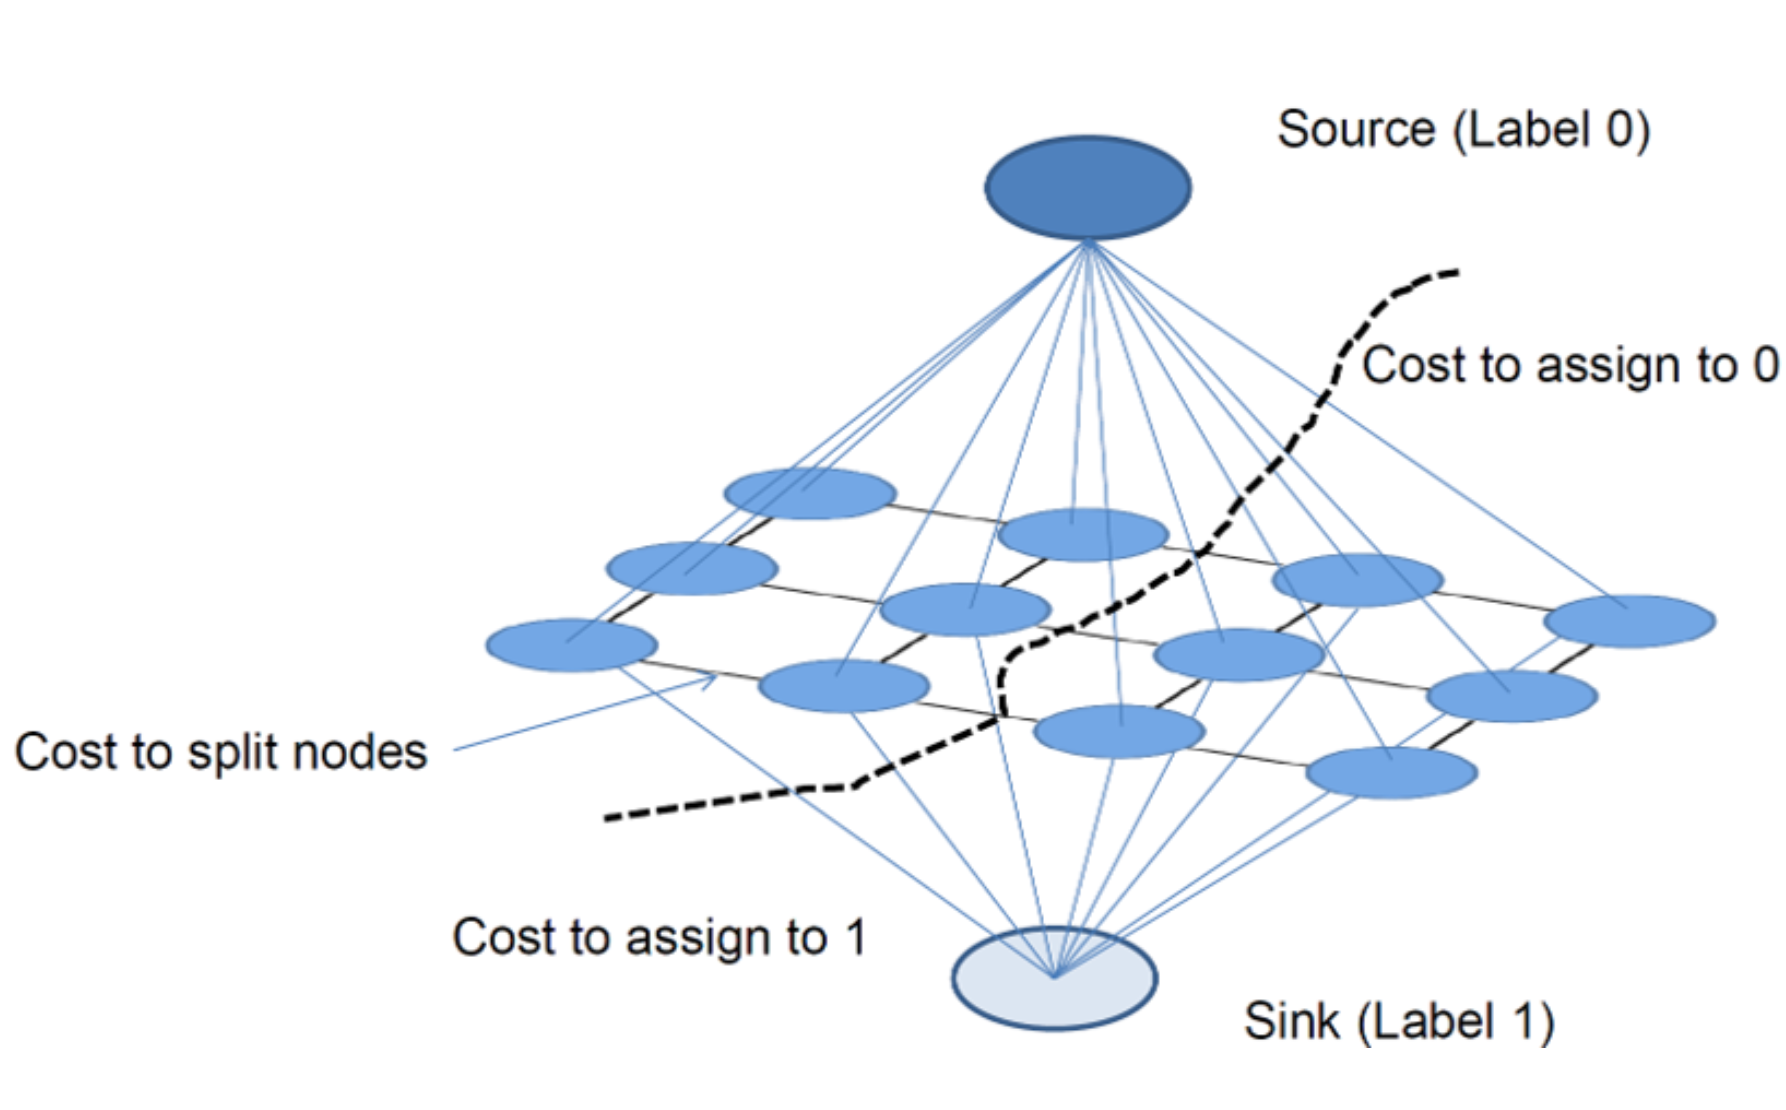
\includegraphics[width=\columnwidth]{segmentation_graph_cut.png}
\section{Fourier Transform}
$$F(u) = \int_{-\infty}^{\infty} f(x)e^{-i2\pi ux} dx,$$

$$f(x) = \int_{-\infty}^{\infty} F(u)e^{i2\pi ux} du$$

$$e^{i2\pi ux} = \cos(2\pi ux) + i\sin(2\pi ux)$$
F(u) holds the amplitude and phase of the corresponding sinusoid.
Amplitude/Magnitude: $A(u) = |F(u)| = \sqrt{(\Re\{F(u)\})^2 + (\Im\{F(u)\})^2}.$

Phase:$\phi(u) = \arg F(u) = \tan^{-1}\left(\frac{\Im\{F(u)\}}{\Re\{F(u)\}}\right)$\\
$$F(u, v) = \int_{-\infty}^{\infty} \int_{-\infty}^{\infty} f(x, y)e^{-i2\pi(ux+vy)} dx\, dy,$$

$$f(x, y) = \int_{-\infty}^{\infty} \int_{-\infty}^{\infty} F(u, v)e^{i2\pi(ux+vy)} du\, dv$$
2d basis function: $$e^{i2\pi(ux+vy)} = \cos(2\pi(ux+vy)) + i\sin(2\pi(ux+vy))$$\\
Basis function has maximal real value when $ux+vy \in \mathbb{N}$. Places where this holds form a line in 2d space characterized by normal vector $(u,v)$.
The distance between two lines (wavelength) is $\frac{1}{\sqrt{u^2+v^2}}$, frequency is inverse.
$u$ and $v$ determine frequency and orientation of the basis function. Pluggin $u,v$ into the Fourier transform of the functiion gives a complex number from which the phase and amplitude can be extracted.
\begin{itemize}
  \item \textbf{Magnitude spectrum} tells you how much of each frequency is present (energy distribution).
  \item \textbf{Phase spectrum} tells you how those frequencies are aligned in space, and this is what gives an image its actual structure.
\end{itemize}
\textbf{Convolution theorem}:$$f(x,y) * h(x,y) \iff F(u,v) \cdot H(u,v)(\text{(element wise)})$$



\section{Sampling}
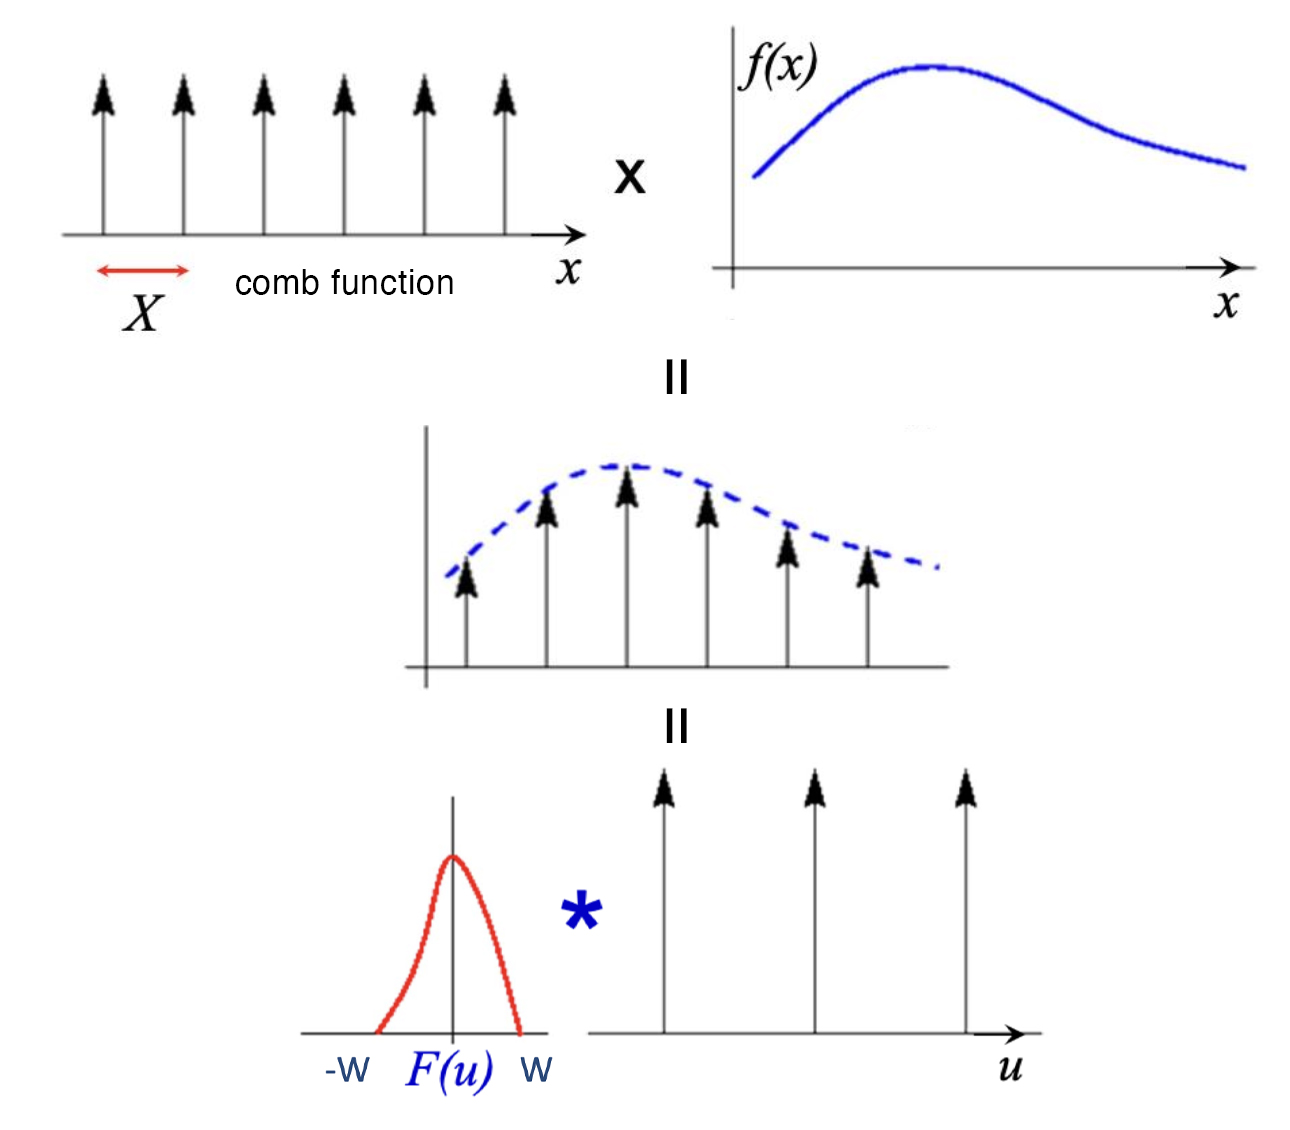
\includegraphics[width=\columnwidth]{sampling.jpg}\\
As the comb samples get further apart, the frequency samples get closer together.\\
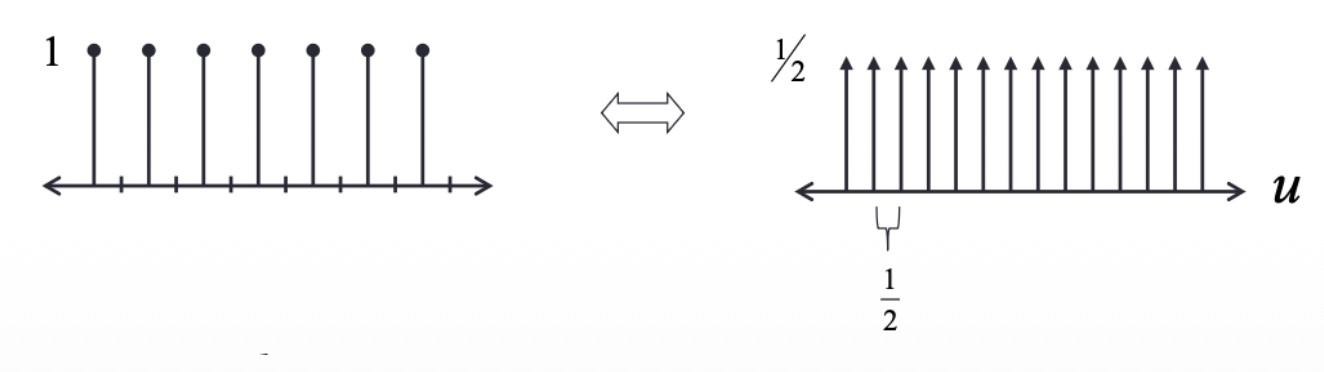
\includegraphics[width=\columnwidth]{Screenshot 2026-01-28 at 15.30.42.png}
\begin{subbox}{Nyquist theorem}
  $f_{\max} \cdot 2 \le 1/x=\text{sampling rate}$
Bc of the convolution theorem it holds: $f_\text{comb} \cdot f_\text{spatial} = f_\text{comb} *F(u) (= f_\text{frequency})$
\end{subbox}


\section{Optical Flow}
We assume brightness constancy. Let I(x,y,t) be the image brightness at location (x,y) at time t. Then:
\begin{align*}
I(x,y,t)&=I(x+\frac{dx}{dt}\delta t , y+\frac{dy}{dt}\delta t ,t+\delta t)\\
&\overset{\text{taylor}}{\approx} I(x, y, t) + \frac{\partial I}{\partial x} \cdot \frac{dx}{dt}\delta t + \frac{\partial I}{\partial y} \cdot \frac{dy}{dt}\delta t + \frac{\partial I}{\partial t} \cdot \delta t\\
&\implies \frac{\partial I}{\partial x}\frac{dx}{dt} + \frac{\partial I}{\partial y}\frac{dy}{dt} + \frac{\partial I}{\partial t} = 0
\end{align*}
To linearize $I$ using Taylor expansion we assume the motion is small from frame to frame.
Denoting $\frac{\partial I}{\partial x}, \frac{\partial I}{\partial y}, \frac{\partial I}{\partial t}$ as $I_x, I_y, I_t$ respectively, and $\frac{dx}{dt}, \frac{dy}{dt}$ as $u, v$, the equation is commonly written as\\
$I_x \cdot u + I_y \cdot v + I_t = 0$
\subsection{Horn-Schunk Algorithm}
Since neighboring pixels tend to move similarly we can add a smoothness constraint. 
\begin{mainbox}{Global Smoothness}
Let $u_x$
denote the change of u in x direction, and so on for $u_y, v_x, v_y$. We then define the smoothness erro as:
$$e_s:=\iint u_x^2+u_y^2+v_x^2+v_y^2dxdy$$
\end{mainbox}
Denoting $e_c:=\iint (I_xu+I_yv+I_t)^2dxdy$, the algorithm focuses on minimizing the combined error $e:=e_c+\lambda e_s$ where $\lambda$ is a weighting factor.
It is minmized using iterative methods with finite differences.
\subsection{Lukas-Kanade Algorithm}
This algorithm aims to enforce consistency in small patches. 
We assume a single velocity for all pixels in a patch $\Omega$. And minimize:
$\sum_{(x,y)\in \Omega}(I_x(x,y)u+I_y(x,y)v+I_t(x,y))^2$ whose least squares solution is given by solving the system:
$$
\begin{bmatrix}
\sum I_x^2 & \sum I_x I_y \\
\sum I_x I_y & \sum I_y^2
\end{bmatrix}
\begin{bmatrix}
u \\
v
\end{bmatrix}
= -
\begin{bmatrix}
\sum I_x I_t \\
\sum I_y I_t
\end{bmatrix}
$$
Sometimes there isn't a unique solution to the system, like when a patch contains only an edge moving to the right with no corner visible (gradient in one direction is zero).\\
The algorithm fails however if the intensity structure in the patch is insufficient (e.g. flat region, edge) or the movement is too large.
To mitigate these issues the algorithm is run on increasingly finer scales of the image with the previous coarser scale's flow used as initialization for the next finer scale. 
\section{Convolution and Filtering}
\section{General Graphics}
Graphics Pipeline Stages:\\
\begin{tabularx}{\columnwidth}{|l|X|}
\hline
Modeling Transform & Transforms objects from their local object space to world space by applying translation, rotation, and scaling operations. \\
\hline
Viewing Transform & Transforms objects from world space to camera/view space, positioning them relative to the camera's viewpoint. \\
\hline
Primitive Processing & Processes geometric primitives (triangles, lines, points) and prepares them for the rendering pipeline. \\
\hline
3D Clipping & Clips geometry against the view frustum to remove parts of primitives that fall outside the visible region. \\
\hline
Projection to Screen Space & Projects 3D coordinates onto a 2D screen space using perspective or orthographic projection. \\
\hline
Scan Conversion & Rasterizes geometric primitives into fragments/pixels, determining which pixels are covered by each primitive. \\
\hline
Lighting, Shading, Texturing & Calculates the color of each fragment based on lighting models, applies shading computations, and maps textures onto surfaces. \\
\hline
Occlusion Handling & Determines visibility using depth testing (z-buffering) to ensure that closer objects obscure farther ones. \\
\hline
Display & Outputs the final rendered image to the screen/framebuffer for presentation. \\
\hline
\end{tabularx}
\section{Programmer's View}
\begin{tabularx}{\columnwidth}{|l|X|}
\hline
Vertex Processing & Performs per-vertex operations including model transformations, lighting, and flow control. \\
\hline
Rasterization & Converts geometric primitives into fragments; interpolates vertex attributes (e.g., colors, texture coordinates) to generate per-pixel inputs for the fragment shader. \\
\hline
Fragment Processing & Performs per-fragment operations such as shading, texturing, and blending to determine the final pixel color. \\
\hline
Display & Outputs the processed fragments to the framebuffer for final display. \\
\hline
\end{tabularx}
Vertex Shader example\\
\begin{verbatim}
uniform mat4 modelViewMatrix;
uniform vec3 lightPosition;
attribute vec3 pos;
attribute vec3 vertexNormal;
varying vec3 lightDirection, normal;
void main() {
  vec4 vertexPosition = modelViewMatrix * pos;
  lightDirection = vec3(lightPosition - vertexPosition);
  normal = vertexNormal;
  gl_Position = vertexPosition;
}
\end{verbatim}

\section{Light and Color}
Light is a electromagnetic radiation at Frequency (wavelength $400 nm$ to $700 nm$).
Spectral Power Distribution: \\ 
$P(\lambda)=\text{intensity at wavelength }\lambda$.\\
Our eye has 3 types of cones (S (blue),M (green),L (red)) with different sensitivity curves. Eye projects $P(\lambda)$ into 3D subspace
using these three basis functions/vectors (two diffrent SPD might look exactly the same to us).\\
\subsection{CIE}
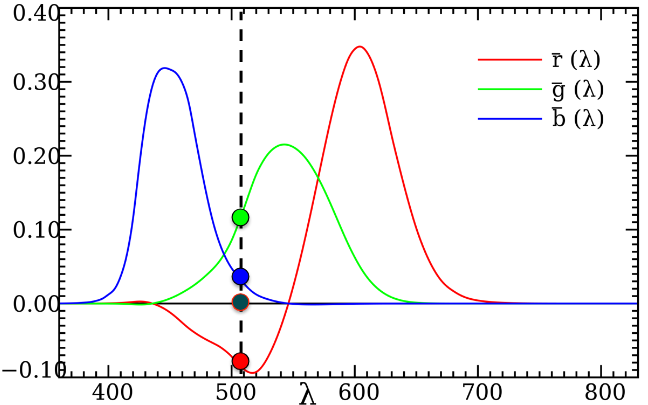
\includegraphics[width=0.6\columnwidth]{CIE_graph.png}\\
$435.8, 546.1$ and $700.0 nm$ (arbitrary choosen) where controlled (dimmed/increased) by observers to match a simulus color. Result is seen above, $x$ is frequency and $y$ is the dimmed strength that the participents did.
Negativ light is not physically possible, was added bc participents could not recreate this color with just red, green and blue.\\
\begin{align*}
 \text{reference} &=  \text{blue} + \text{green} - \text{red}\\
 \text{reference} + \text{red} &= \text{blue} + \text{green}
\end{align*}

\subsection{CIE-XYZ/xyY color space}
choosing the $\hat{r}, \hat{g}, \hat{b}$ basis is fairly arbitrary, to avoid negative values we can define a new basis:
\begin{align*}
\begin{pmatrix}
\bar{x}(\lambda) \\ 
\bar{y}(\lambda) \\ 
\bar{z}(\lambda)
\end{pmatrix} 
&= 
\begin{pmatrix} 
2.36 & -0.515 & 0.005 \\ 
-0.89 & 1.426 & 0.014 \\ 
-0.46 & 0.088 & 1.009 
\end{pmatrix} 
\begin{pmatrix} 
\bar{r}(\lambda) \\ 
\bar{g}(\lambda) \\ 
\bar{b}(\lambda) 
\end{pmatrix}\\
X &= \int_{0}^{\infty} P(\lambda)\bar{x}(\lambda)d\lambda \\
Y &= \int_{0}^{\infty} P(\lambda)\bar{y}(\lambda)d\lambda \\
Z &= \int_{0}^{\infty} P(\lambda)\bar{z}(\lambda)d\lambda \\
x &= \frac{X}{X + Y + Z} \\
y &= \frac{Y}{X + Y + Z}
\end{align*}
While Y describes brightness, x and y describe color and give us the  CIE chromaticity chart:\\
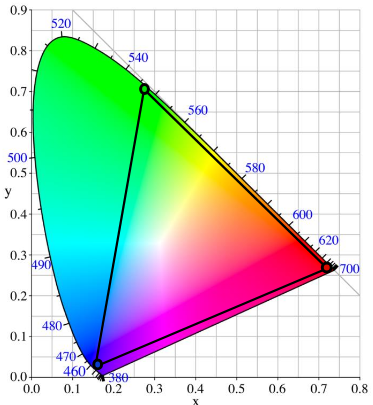
\includegraphics[width=0.5\columnwidth]{cie_horsesho.png}\\
\begin{itemize}
  \item Primary colors are along the edge of the horseshoe
  \item linear combinations of colors are along straight lines
  \item linear combinations of 3 colors form a triangle
\end{itemize}
\subsection{CMY color space}
\begin{itemize}
    \item \textbf{Passive Systems:} Used for printers (subtractive mixing).
    \item \textbf{Inverse to RGB:}
    \[
    \begin{bmatrix} C \\ M \\ Y \end{bmatrix} = \begin{bmatrix} 1 \\ 1 \\ 1 \end{bmatrix} - \begin{bmatrix} R \\ G \\ B \end{bmatrix}
    \]
    \item \textbf{CMYK:} Adds \textbf{Black (K)} to improve contrast and reduce ink usage.
\end{itemize}
\subsection{YIQ Color Space}
\begin{itemize}
    \item \textbf{Components:} Luminance ($Y$), In-phase ($I$, orange-blue, Humans are very sensitive to this so it got more bandwidth), Quadrature ($Q$, purple-green, kind of blind in those colors).
    \item \textbf{Usage:} NTSC (US TV standard); advantageous for natural/skin colors.
    \item \textbf{RGB to YIQ Transformation:}
    \[
    \begin{bmatrix} Y \\ I \\ Q \end{bmatrix} = 
    \begin{bmatrix} 
    0.299 & 0.587 & 0.114 \\ 
    0.596 & -0.275 & -0.321 \\ 
    0.212 & -0.523 & 0.311 
    \end{bmatrix} 
    \begin{bmatrix} R \\ G \\ B \end{bmatrix}
    \]
\end{itemize}
\subsection{HSV \& HSL/HSB Color Spaces}
\begin{itemize}
    \item \textbf{Concept:} User-oriented and intuitive (painters/designers); separates color info ($H, S$) from intensity ($V$).
    \item \textbf{Geometry:} Derived by projecting the RGB Cube onto a hexagon (forming a Hexcone).
    \item \textbf{Dimensions:}
    \begin{itemize}
        \item \textbf{Hue (H):} The "base color" (angle on the hexagon, $0^\circ-360^\circ$).
        \item \textbf{Saturation (S):} Purity/Richness (radius from center; $0$ = gray).
        \item \textbf{Value (V):} Brightness/Lightness (vertical axis).
    \end{itemize}
    \item \textbf{RGB $\to$ HSV Conversion:} code TODO.\\
\end{itemize}
\subsection{CIELAB and CIELUV Color Spaces}
moving on the horseshoe changes the perceived color difference non-linearly (sometimes tini movement and big change in precived color, sometimes the oposit). To fix this we can define a new color space where euclidean distances correspond to perceived color differences. 
\subsection{high dinamic range (HDR)}
take multiple images at different exposures and combine them to get a higher dynamic range.


\section{Miscallaneous}
\begin{itemize}
    \item $e^{i\pi} + 1 = 0$
    \item $e^{i2\pi ux} = \cos(2\pi ux) + i\sin(2\pi ux)$
    \item $e^{i2\pi ux} = \cos(2\pi ux) + i\sin(2\pi ux)$
    \item $e^{-i2\pi ux} = \cos(-2\pi ux) + i\sin(-2\pi ux)$
    \item $\cos(2\pi ux) = \frac{e^{i2\pi ux} + e^{-i2\pi ux}}{2}$
    \item $\sin(2\pi ux) = \frac{e^{i2\pi ux} - e^{-i2\pi ux}}{2i}$
\end{itemize}
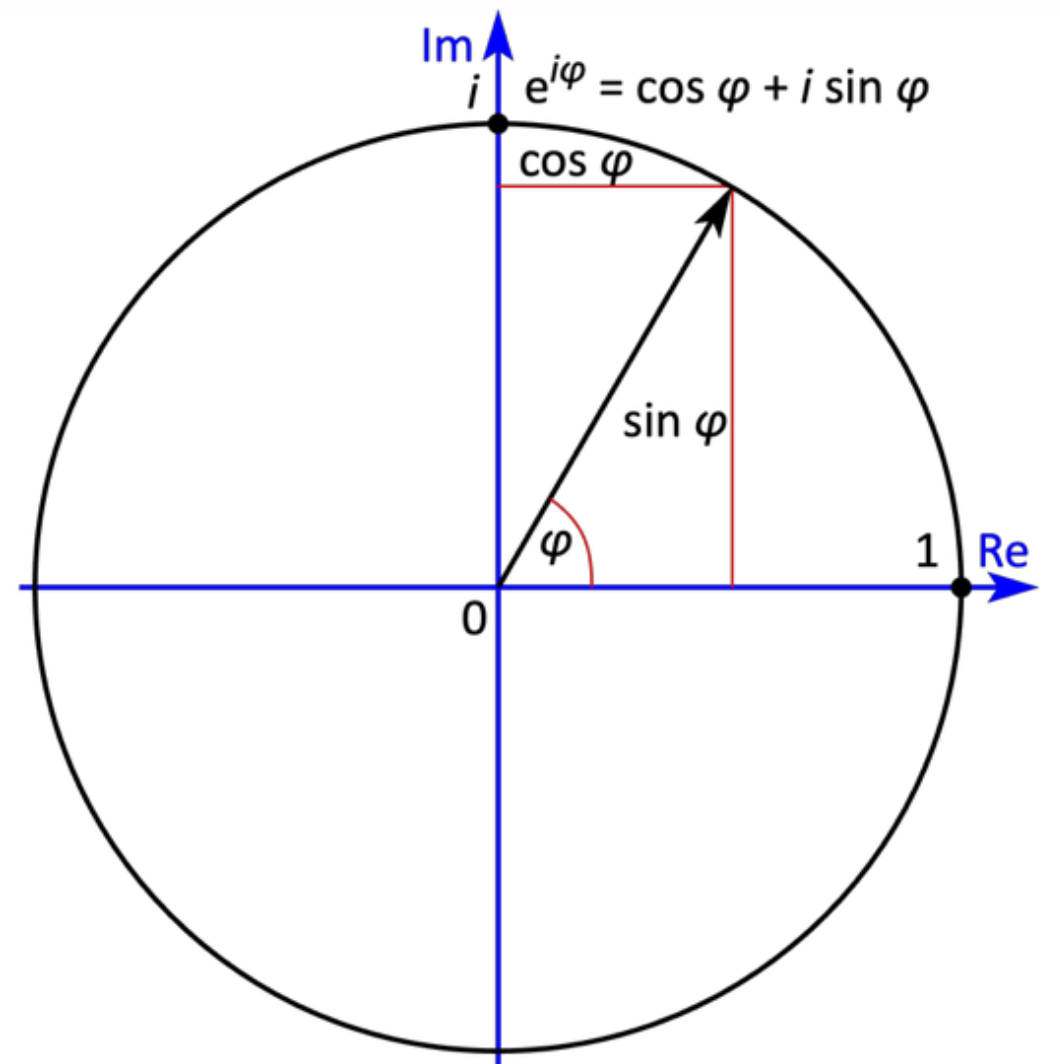
\includegraphics[width=0.5\columnwidth]{Screenshot 2026-01-28 at 13.22.38.png}
\end{document}

